
\section{Entrenamiento de una RNA}


\begin{frame}
	\frametitle{Backpropagation: Corrección de erroes}
	\begin{center}
		\begin{tikzpicture}[scale=0.7, transform shape, >=Stealth]
			% Estilos de nodos
			\tikzset{
				neuron/.style={circle,fill=black!25,minimum size=22pt,inner sep=0pt},
				input neuron/.style={neuron, fill=green!50},
				output neuron/.style={neuron, fill=red!50, align=center},
				hidden neuron/.style={neuron, fill=blue!50, align=center},
				annot/.style={text width=4em, text centered}
			}
			
			% Dibuja la capa de entrada
			\foreach \name / \y in {1,...,2}
			\node[input neuron] (I-\name) at (0,-\y*2.5) {$x_{\name}$};
			
			% Dibuja la capa oculta
			\foreach \name / \y in {1,...,3}
			\node[hidden neuron] (H-\name) at (5cm,-\y*2.5) {$\sigma$};
			
			% Dibuja la capa de salida
			\node[output neuron,pin={[pin edge={->}]right:$\hat{y}$}, right=of H-2] (O) {$\sigma$};
			
			% Conecta las unidades con pesos
			\foreach \source in {1,...,2} {
				\foreach \dest in {1,...,3} {
					\draw (I-\source) -- (H-\dest) node[midway, above, sloped, pos=0.7, xshift=(\source-1.5)*3pt, yshift=(\dest-2)*3pt] {$w_{\source,\dest}$};
				}
			}
			
			% Conecta la capa oculta a la de salida con pesos
			\foreach \source in {1,...,3} {
				\pgfmathtruncatemacro{\result}{\source}
				\draw (H-\source) -- (O) node[midway, above, sloped, yshift=\source*2pt] {$w_{\result,1}$};
			}
			
			% Etiquetas
			\node[annot,above=of H-1, yshift=0.1cm] {Capa oculta};
			\node[annot,left=of I-1, node distance=3cm] (capa_entrada) {Capa de entrada};
			\node[annot,right=of O, node distance=3cm] {Capa de salida};
			
			% Dibuja el vector columna debajo de la etiqueta "Capa de entrada"
			\node[below=0.5cm of capa_entrada] (vector) {${\vec{\mathbf{X}}} = \begin{bmatrix} x_1 \\ x_2 \\ \vdots \\ x_n \end{bmatrix}$};
			
			% Conexiones de vector columna
			\draw[->] (vector) -- (I-1);
			\draw[->] (vector) -- (I-2);
			
			% Sesgo
			\node[above=0.5cm of H-2] (Bias) {$b$};
			\draw[->] (Bias) -- (H-2);
			
			% Flecha "forward"
			% Flecha "Forward" controlada manualmente
			\draw[->, thick] (8, -9) -- node[above] {Backpropagation} (-1, -9);
		\end{tikzpicture}
	\end{center}
	
	
\end{frame}


\begin{frame}
	\frametitle{Función de Error (MSE)}
	
	\textbf{MSE: Mean Square Error}
	
	\begin{block}{Expresión Matemática}
		La fórmula para calcular el MSE es:
		\[ MSE = \frac{1}{n} \sum_{i=1}^{n} (Y_{i} - \hat{Y}_{i})^2 \]
		donde:
		\begin{itemize}
			\item $n$ es el número total de observaciones (o ejemplos de entrenamiento),
			\item $Y_{i}$ es el valor real del i-ésimo ejemplo,
			\item $\hat{Y}_{i}$ es la predicción del modelo para el i-ésimo ejemplo.
		\end{itemize}
	\end{block}
	
\end{frame}

\begin{frame}
	\frametitle{Función de Error (MSE)}
	\begin{block}{Explicación: ¿Qué hace el MSE?}
		El MSE mide el promedio de los cuadrados de los errores; es decir, la diferencia cuadrática promedio entre los valores estimados y los valores reales. Al elevar al cuadrado las diferencias:
		\begin{itemize}
			\item Penaliza más fuertemente los errores grandes, lo que puede ser deseable en muchos casos.
			\item Asegura que solo tengamos valores positivos, simplificando el análisis de los errores.
		\end{itemize}
		Esto lo convierte en una herramienta poderosa para guiar al modelo en el proceso de aprendizaje, buscando minimizar estas diferencias y, por ende, el error de predicción.
	\end{block}
\end{frame}

\begin{frame}
	\frametitle{Función de Error (MSE)}
	\begin{block}{¿Por qué es importante el MSE?}
		Una función de error baja indica que el modelo tiene una buena precisión en sus predicciones. Reducir el MSE es fundamental en el proceso de optimización del modelo, llevándolo a hacer predicciones cada vez más cercanas a los valores reales.
	\end{block}
\end{frame}

\begin{frame}
	\frametitle{Resumen}
	
	\begin{table}[h]
		\centering
		\begin{tabular}{|l|p{6cm}|c|}
			\hline
			Elemento & Descripción & Origen \\ \hline
			Entradas ($\vec{x}$) & Variables de entrada proporcionadas al modelo (por ejemplo, características de los datos de entrada) & P \\ \hline
			Pesos ($\vec{\mathbf{W}}$) & Parámetros aprendidos por el modelo durante el entrenamiento & C \\ \hline
			Sesgo ($\vec{b}$) & Término aditivo introducido para ajustar la salida de cada neurona & P \\ \hline
			Función de activación & Función aplicada a la salida de cada neurona para introducir no linealidades en el modelo & P \\ \hline
		\end{tabular}
		\caption{Elementos básicos de una red neuronal (Parte 1)}
		\label{table:elementos_red_neuronal1}
	\end{table}
	
\end{frame}

\begin{frame}
	\frametitle{Resumen}
	
	\begin{table}[h]
		\centering
		\begin{tabular}{|l|p{6.5cm}|c|}
			\hline
			Elemento & Descripción & Origen \\ \hline
			Función de error & Función que mide la discrepancia entre las predicciones del modelo y los valores reales & P \\ \hline
			Capas ocultas & Capas intermedias entre la capa de entrada y la capa de salida que contienen neuronas & P \\ \hline
			Neuronas por capa & Número de unidades de procesamiento en cada capa oculta & P \\ \hline
			Predicción ($\hat{y}$) & Valor calculado por el modelo como salida final & C \\ \hline
			Target ($y$) & Valor real al que se compara la predicción durante el entrenamiento & P \\ \hline
		\end{tabular}
		\caption{Elementos básicos de una red neuronal (Parte 2)}
		\label{table:elementos_red_neuronal2}
	\end{table}
\end{frame}

\begin{frame}
	\frametitle{Resumen}
	\begin{center}
		{\large Entrenar una Red Neuronal implica aplicar el método de \textit{Prueba y Error}. Es un algoritmo que nos puede ayudar a dominar el arte de tener paciencia.}
		
		\vspace{5mm}
		
		
\includegraphics[width=3.8cm]{cerveza.jpg}
		
	\end{center}
	
\end{frame}


\begin{frame}
	\frametitle{Entrenamiento de una RNA}
	
	\textit{\textbf{Objetivo:} Minimizar la función de error.}
	\vspace{3mm}
	
	¿CÓMO?
	\vspace{3mm}
	
	\begin{itemize}
		\item Aplicando derivadas
		\item Para el caso de una función multivariable: \textbf{Aplicando el gradiente}
		\item Como es difícil usar un método analítico (con fórmulas) para determinar el mínimo de la función de error:
		\begin{itemize}
			\item Aplicamos un método numérico iterativo conocido como: \textit{\textbf{Descenso de gradiente.}}
		\end{itemize}
	\end{itemize}
        
 
\end{frame}

%------------------------------------------------

\begin{frame}
	\frametitle{Descenso de gradiente - El parámetro learning\_rate ($\alpha$)}
	
     \begin{center}
     	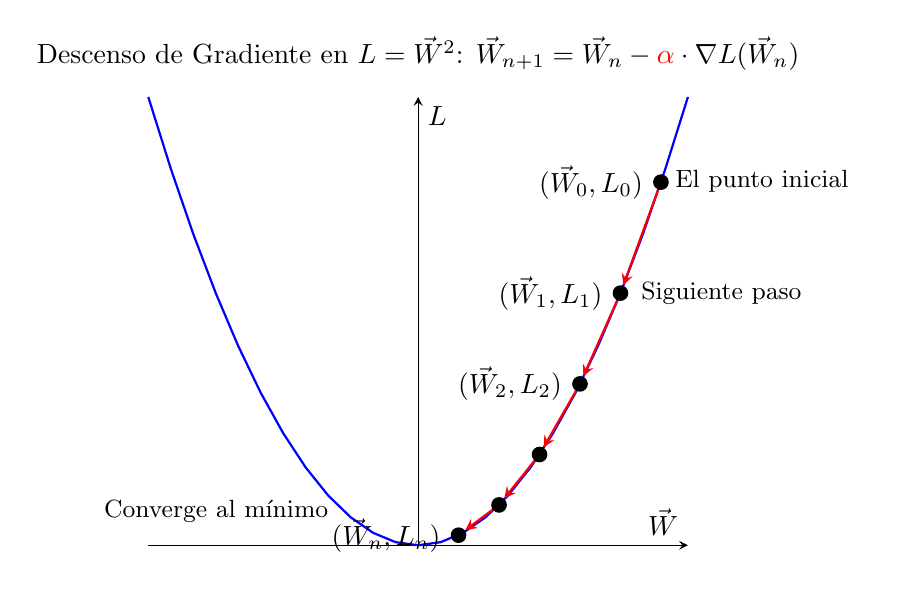
\begin{tikzpicture}
     		\begin{axis}[
     			title={Descenso de Gradiente en $L = \vec{W}^2$: $\vec{W}_{n+1} = \vec{W}_n - \textcolor{red}{\alpha} \cdot \nabla L(\vec{W}_n)$},
     			xlabel={$\vec{W}$},
     			ylabel={$L$},
     			axis lines=middle,
     			xmin=-2, xmax=2,
     			ymin=0, ymax=4,
     			ticks=none,
     			clip=false,
     			]
     			
     			% Dibuja la función
     			\addplot[blue, thick, domain=-2:2] {x^2};
     			
     			% Puntos y flechas del descenso de gradiente
     			\node<2->[label={180:{$(\vec{W}_0,L_0)$}},circle,fill,inner sep=2pt] (start) at (axis cs:1.8,{1.8^2}) {};
     			\node<3->[label={180:{$(\vec{W}_1,L_1)$}},circle,fill,inner sep=2pt] (mid1) at (axis cs:1.5,{1.5^2}) {};
     			\node<4->[label={180:{$(\vec{W}_2,L_2)$}},circle,fill,inner sep=2pt] (mid2) at (axis cs:1.2,{1.2^2}) {};
     			\node<5->[circle,fill,inner sep=2pt] (mid3) at (axis cs:0.9,{0.9^2}) {};
     			\node<6->[circle,fill,inner sep=2pt] (mid4) at (axis cs:0.6,{0.6^2}) {};
     			\node<7->[label={180:{$(\vec{W}_n,L_n)$}},circle,fill,inner sep=2pt] (end) at (axis cs:0.3,{0.3^2}) {};
     			
     			% Flechas entre los puntos
     			\draw<3->[-stealth, red, thick] (start) -- (mid1);
     			\draw<4->[-stealth, red, thick] (mid1) -- (mid2);
     			\draw<5->[-stealth, red, thick] (mid2) -- (mid3);
     			\draw<6->[-stealth, red, thick] (mid3) -- (mid4);
     			\draw<7->[-stealth, red, thick] (mid4) -- (end);
     			
     			% Anotaciones
     			\node<2->[align=center, font=\small, text width=3cm, anchor=west] at (axis cs:1.6,3.25) 
     			{El punto inicial};
     			\node<3->[align=center, font=\small, text width=3cm, anchor=west] at (axis cs:1.3,2.25) 
     			{Siguiente paso};
     			\node<7->[align=center, font=\small, anchor=west] at (axis cs:-2.4,0.3) 
     			{Converge al mínimo};
     			
     		\end{axis}
     	\end{tikzpicture}
     \end{center}
 
\end{frame}

%------------------------------------------------

\begin{frame}
	\frametitle{Cuando $\alpha$ es muy pequeño}
	
	\begin{center}
		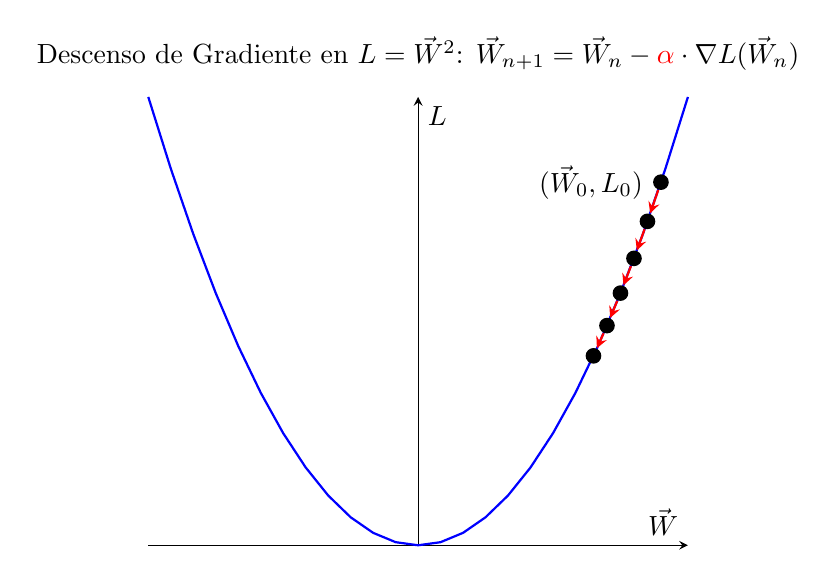
\begin{tikzpicture}
			\begin{axis}[
				title={Descenso de Gradiente en $L = \vec{W}^2$: $\vec{W}_{n+1} = \vec{W}_n - \textcolor{red}{\alpha} \cdot \nabla L(\vec{W}_n)$},
				xlabel={$\vec{W}$},
				ylabel={$L$},
				axis lines=middle,
				xmin=-2, xmax=2,
				ymin=0, ymax=4,
				ticks=none,
				clip=false,
				]
				
				% Dibuja la función
				\addplot[blue, thick, domain=-2:2] {x^2};
				
				% Puntos y flechas del descenso de gradiente
				\node[label={180:{$(\vec{W}_0,L_0)$}},circle,fill,inner sep=2pt] (start) at (axis cs:1.8,{1.8^2}) {};
				
				\node[label={180:{}},circle,fill,inner sep=2pt] (mid1) at (axis cs:1.7,{1.7^2}) {};
				
				\node[label={180:{}},circle,fill,inner sep=2pt] (mid2) at (axis cs:1.6,{1.6^2}) {};
				
				\node[label={180:{}},circle,fill,inner sep=2pt] (mid3) at (axis cs:1.5,{1.5^2}) {};
				
				\node[label={180:{}},circle,fill,inner sep=2pt] (mid4) at (axis cs:1.4,{1.4^2}) {};
				
				\node[label={180:{}},circle,fill,inner sep=2pt] (end) at (axis cs:1.3,{1.3^2}) {};
					
				% Flechas entre los puntos
				\draw[-stealth, red, thick] (start) -- (mid1);
				\draw[-stealth, red, thick] (mid1) -- (mid2);
				\draw[-stealth, red, thick] (mid2) -- (mid3);
				\draw[-stealth, red, thick] (mid3) -- (mid4);
				\draw[-stealth, red, thick] (mid4) -- (end);
				
			\end{axis}
		\end{tikzpicture}
	\end{center}"
	
\end{frame}


\begin{frame}
	\frametitle{Cuando $\alpha$ es muy grande}
	
	\begin{center}
		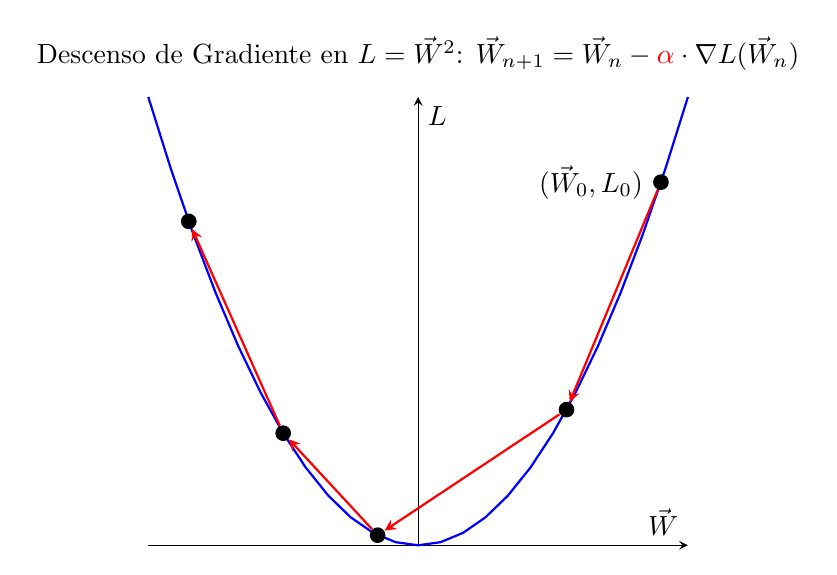
\begin{tikzpicture}
			\begin{axis}[
				title={Descenso de Gradiente en $L = \vec{W}^2$: $\vec{W}_{n+1} = \vec{W}_n - \textcolor{red}{\alpha} \cdot \nabla L(\vec{W}_n)$},
				xlabel={$\vec{W}$},
				ylabel={$L$},
				axis lines=middle,
				xmin=-2, xmax=2,
				ymin=0, ymax=4,
				ticks=none,
				clip=false,
				]
				
				% Dibuja la función
				\addplot[blue, thick, domain=-2:2] {x^2};
				
				% Puntos y flechas del descenso de gradiente
				\node[label={180:{$(\vec{W}_0,L_0)$}},circle,fill,inner sep=2pt] (start) at (axis cs:1.8,{1.8^2}) {};
				
				\node[label={180:{}},circle,fill,inner sep=2pt] (mid1) at (axis cs:1.1,{1.1^2}) {};
				
				\node[label={180:{}},circle,fill,inner sep=2pt] (mid2) at (axis cs:-0.3,{(-0.3)^2}) {};
				
				\node[label={180:{}},circle,fill,inner sep=2pt] (mid3) at (axis cs:-1,{(-1)^2}) {};
				
				\node[label={180:{}},circle,fill,inner sep=2pt] (end) at (axis cs:-1.7,{(-1.7)^2}) {};
				
				
				% Flechas entre los puntos
				\draw[-stealth, red, thick] (start) -- (mid1);
				\draw[-stealth, red, thick] (mid1) -- (mid2);
				\draw[-stealth, red, thick] (mid2) -- (mid3);
				\draw[-stealth, red, thick] (mid3) -- (end);
				
			\end{axis}
		\end{tikzpicture}
	\end{center}
	
\end{frame}

\begin{frame}
	\begin{center}
		Y si... el learning\_rate también lo define el programador /:
		\vspace{5mm}
		
		
\includegraphics[width=6cm]{gato.jpeg}
	\end{center}
\end{frame}

\begin{frame}
	\frametitle{Ejemplito: Compuerta XOR}
	\vspace{-5mm}
	\begin{columns}
		\begin{column}{0.5\textwidth}
			\begin{center}
				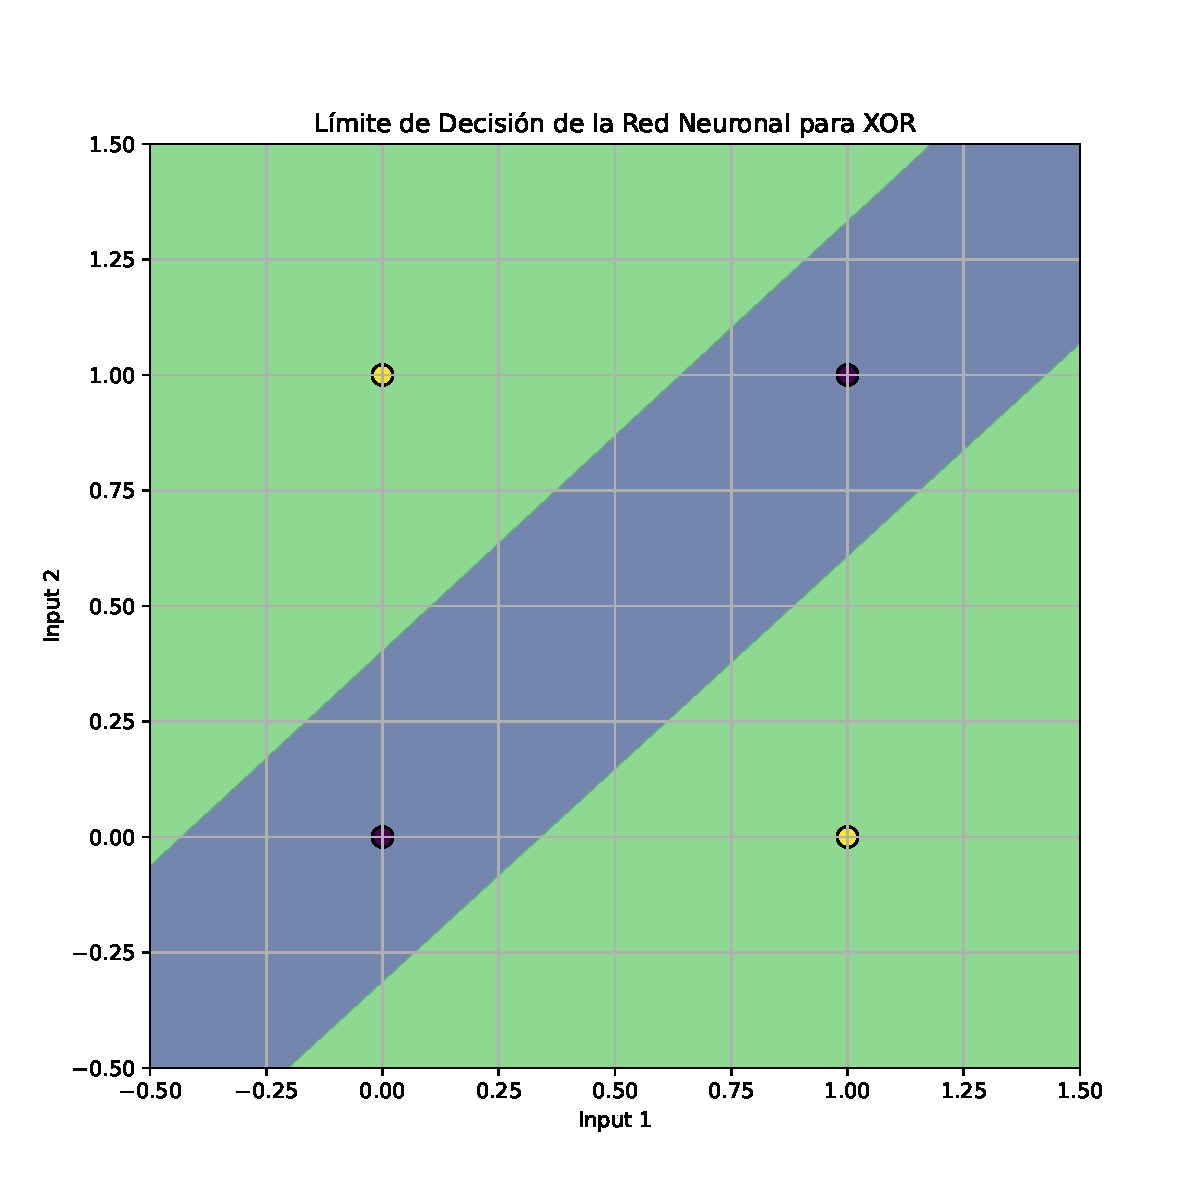
\includegraphics[width=0.6\linewidth]{xor1.pdf}
			\end{center}
		\end{column}
		\begin{column}{0.5\textwidth}
			\begin{center}
				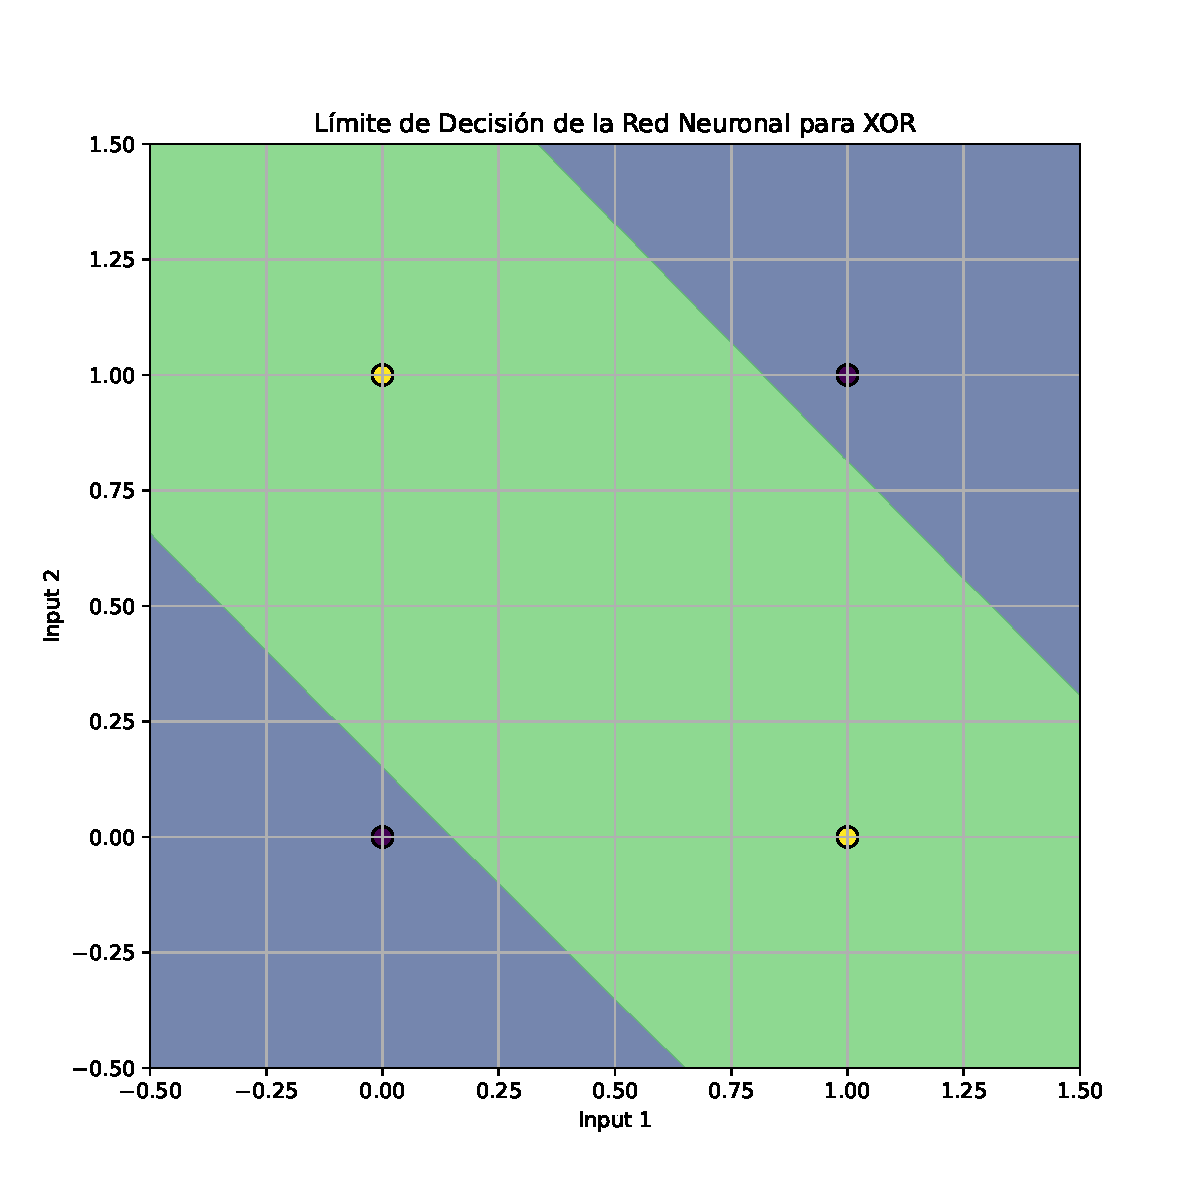
\includegraphics[width=0.6\linewidth]{xor2.pdf}
			\end{center}
		\end{column}
	\end{columns}

	
	\begin{columns}
		\begin{column}{0.5\textwidth}
			\begin{center}
				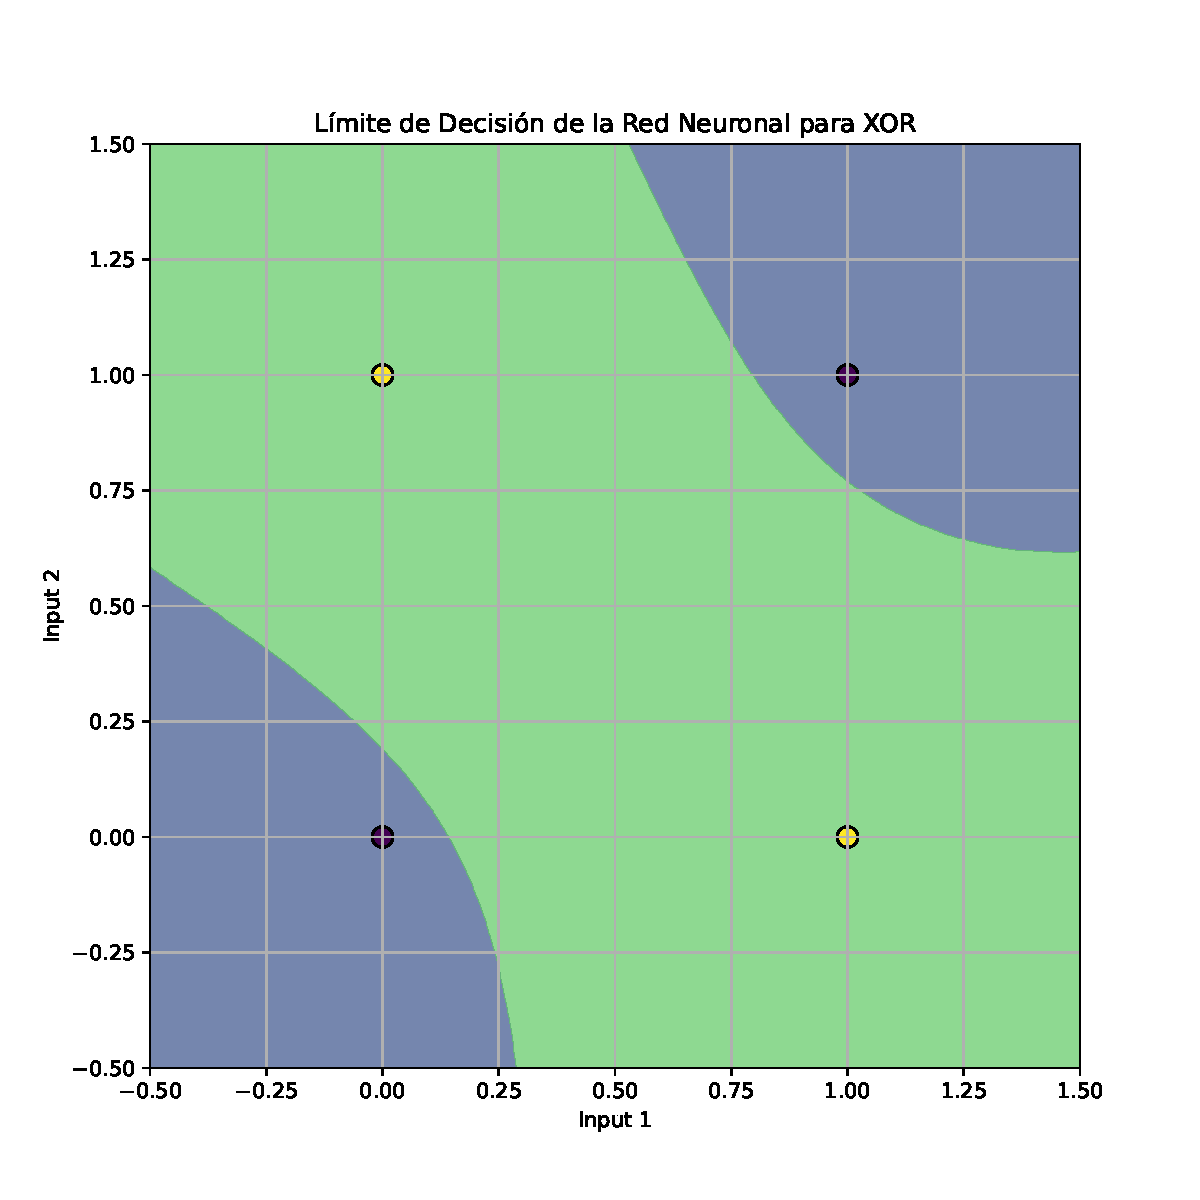
\includegraphics[width=0.6\linewidth]{xor3.pdf}
			\end{center}
		\end{column}
		\begin{column}{0.5\textwidth}
			\begin{center}
				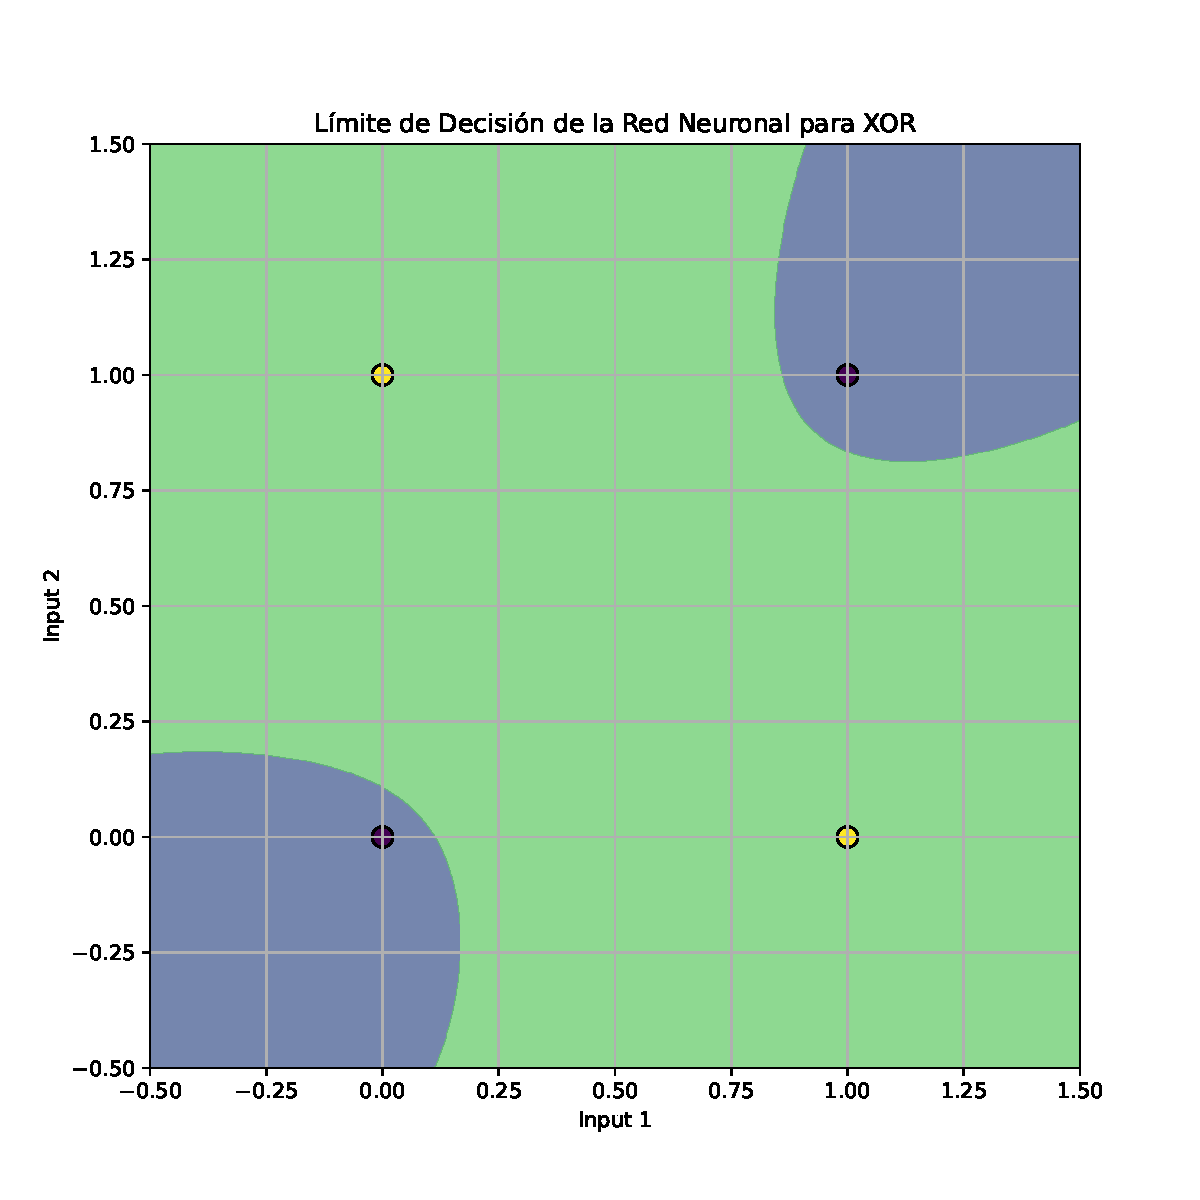
\includegraphics[width=0.6\linewidth]{xor4.pdf}
			\end{center}
		\end{column}
	\end{columns}
\end{frame}
